\section{Experiments}
\label{sec:experiments}
\comment{Zoltan}{The above section 3.4 should be part of this section}

To fully verify the implementation of the proposed architecture, a number of experiments have been conducted. The experiments are designed to test and validate the following aspects of the architecture: 

\begin{description}
    \item[Communication] How does the communication between agents affect the number of adaptations and the number of risks identified?
    \item[Cooperation] How does the cooperation between agents affect the number of adaptations and the number of risks identified?
\end{description}

The experiments are conducted in a simulated environment, where the agents are connected to a \code{ExperimentManager} which is responsible for creating the infrastructure, \comment{Zoltan}{is this really done by the ExperimentManager}managing the communication between agents, starting the experiment, and stopping the experiment after a predefined number of epochs\footnote{Epochs are further explained in REFERENCE}. The \code{ExperimentManager} is also responsible for measuring metrics as explained in Section \ref{ssec:metrics}. \comment{Zoltan}{I think that shouldn't matter}The experiments are conducted in the following order:

\begin{enumerate}
    \item Baseline experiment
    \item Experiment 1: Risk Analysis 
    \item Experiment 2: Risk Mitigation 
\end{enumerate}

\comment{Zoltan}{It's worth emphasizing that the experiments are conducted in a simulated environment.}
Each of the experiments is performed on the same infrastructure, but with different configurations. \tocheck{Update this depending on the final infrastructure} The infrastructure is a simple network consisting of 4 nodes, where each node has 4 software components. The nodes are connected as shown in Figure \ref{fig:infrastructure}. The infrastructure is created by the \code{ExperimentManager} and is the same for all experiments.

\begin{figure}[H]
    \centering
    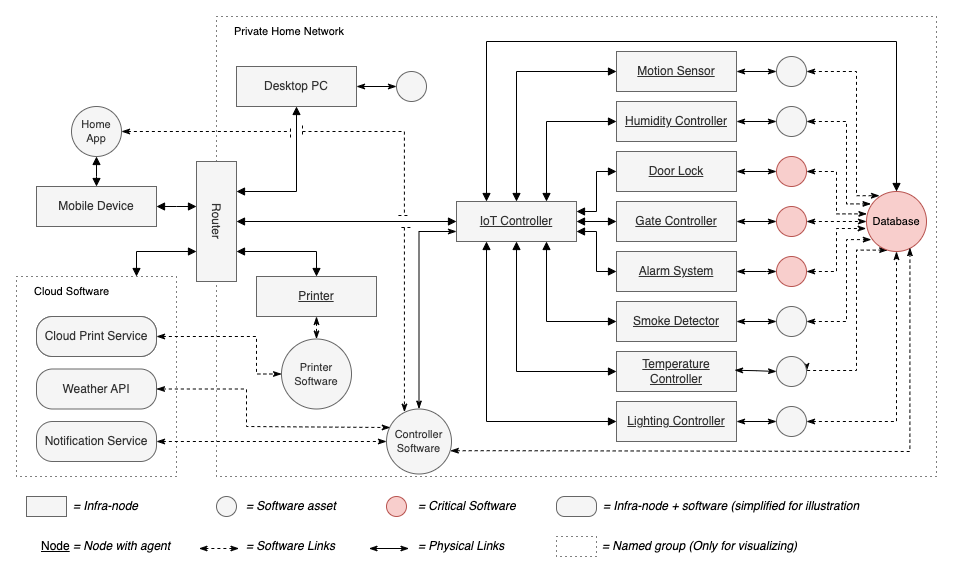
\includegraphics[width=0.8\textwidth]{_content/infrastructure}
    \caption{Experiment Infrastructure.}
    \label{fig:infrastructure}
\end{figure}
\comment{Zoltan}{What do the arrows mean? I think they might have different meaning, depending on whether they connect two nodes or a node and a SW Component}

\subsection{Baseline Experiment}
% - No communication, no cooperation
% - Predefined Infrastructure, same as other experiments
% - Measure:
%   - Number of adaptations
%   - Total number of risks identified
%   - Number of remaining risks
%   - Sum of the damage for remaining risks

% Mitigations take time, also communication. This should be discussed and used in the experiment.
% Check costs of a mitigation

\comment{Zoltan}{Arent these metrics collected in all experiments}The baseline experiment is conducted to measure metrics such as the number of adaptations and the number of risks identified. In this experiment Agents are not able to communicate with each other, and are not able to cooperate. 

When the experiment has started, the agents are allowed to adapt their own properties and software components. However, the agents are not able to share knowledge and otherwise communicate with each other. To make the experiment easier to manage the \code{ExperimentManager} still is able to send messages to the agents, but the agents are not able to send messages to each other. \comment{Zoltan}{and also not able to cooperatively discover risks that require a global view I guess} Agents to being able to cooperate means that they are not able to join in auctions and therefore not able to work together to mitigate risks. A schematic overview of the experiment is shown in Figure \ref{fig:baseline}.

\begin{figure}[H]
    \centering
    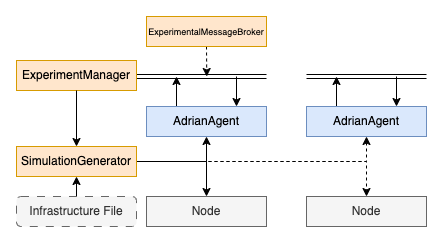
\includegraphics[width=0.8\textwidth]{_content/adrian-experiment-0}
    \caption{Schematic overview of the baseline experiment, where multiple Agents are disconnected from one another.}
    \label{fig:baseline}
\end{figure}
\comment{Zoltan}{It's not fully clear what this figure conveys. What do the individual symbols mean? In general, it is a good idea to explain all figures in the text, because they are often not as self-explanatory as you might think.}

\subsection{Experiment 1: Risk Analysis (communication)}
% - Communication, no cooperation
% - Predefined Infrastructure, same as other experiments
% - Measure:
%   - Number of adaptations
%   - Total number of messages exchanged
%   - Total number of risks identified
%   - Number of remaining risks
%   - Sum of the damage for remaining risks

The first experiment is conducted to measure the effect of communication between agents. In this experiment agents are able to communicate with each other, \comment{Zoltan}{I think you mean this only for mitigation, not for risk identification?} but are not able to cooperate. 

When the experiment has started, the agents are allowed to adapt their own properties and software components. The agents are also able to share knowledge at a distance of \( D_{knowledge} \). In this experiment Agents are still not able to cooperate on mitigating risks, which is achieved by not allowing Agents to initiate or join auctions. A simplified overview of the experiment is shown in Figure \ref{fig:experiment-1}.

\begin{figure}[H]
    \centering
    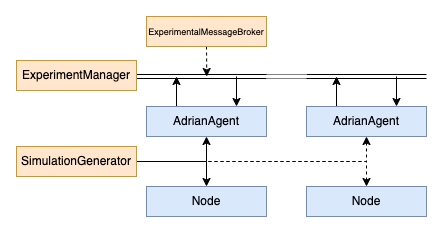
\includegraphics[width=0.8\textwidth]{_content/adrian-experiment-1}
    \caption{Schematic overview of the first and second experiment, depicting the way multiple Agents are connected to each other and are controlled by the \code{ExperimentManager}.}
    \label{fig:experiment-1}
\end{figure}
\comment{Zoltan}{It's not easy to spot the difference between this and the previous figure, like in a puzzle. Please make the life of your readers easier.}

This experiment is repeated multiple times, with different values for \( D_{knowledge} \). The values for \( D_{knowledge} \) are 1, 2, and 3. The results of this experiment are compared to the results of the baseline experiment.

\subsection{Experiment 2: Risk Mitigation (cooperation)}
% - Communication, cooperation
% - Predefined Infrastructure, same as other experiments
% - Measure:
%   - Number of adaptations
%   - Total number of messages exchanged
%   - Total number of risks identified
%   - Number of remaining risks
%   - Sum of the damage for remaining risks

The second experiment is conducted to measure the effect of cooperation between agents. In this experiment agents are able to communicate with each other, and are able to cooperate. 

When the experiment has started, the agents are allowed to adapt their own properties and software components. The agents are also able to share knowledge at a distance of \( D_{knowledge} \). Additionally, in this experiment Agents are able to cooperate on mitigating risks, which is achieved by allowing Agents to initiate and join auctions. The overview of this experiment is shown in Figure \ref{fig:experiment-1}.

As with the first experiment, this experiment is repeated multiple times, with different values for \( D_{knowledge} \). The values for \( D_{knowledge} \) are 1, 2, and 3. The results of this experiment are compared to the results of the baseline experiment and the first experiment.
